\chapter{Release Description}

\section{Intended use}
Please review the Statement of Work for specific intended use information.

\section{Functions implemented in this release}
\input{generated/tables/implemented-functions.tex}
   
\section{Functions not implemented in this release}
N/A

\section{Folder structure}
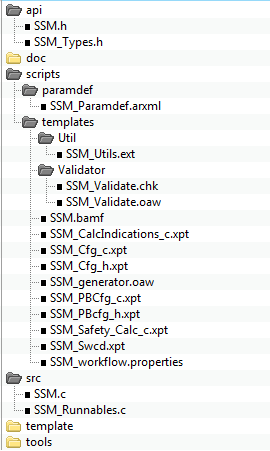
\includegraphics{images/SSM_tree.png}

\section{Release Package Contents}

\subsection{ETAS Developed Software}
\input{generated/tables/released_software_ETAS.tex}

\subsection{Third-party Developed Software}
N/A

\section{Configuration Management Items (Documents only)}
\input{generated/tables/released_documents.tex}
   
\section{Target Environment Description}

\subsection{Hardware Target System and Components}
\begin{tabular}{ |l|l| }
	\hline
	{\bfseries Manufacturer} & {\bfseries}\\ \hline
	Model Number & ISOLAR-EVE\\ \hline
	Description & Virtual development and testing environment\\ \hline
\end{tabular}

\subsection{Software Prerequisites/Dependencies}
\begin{itemize}
\item In Loss communication with provider functionality, fault signals are monitored for TimeOut, which sets the ECU to Lost Communication. This is necessary for setting both \code{ComFirstTimeout} and \code{ComTimeout} Com Parameters, as required for Loss of Commmunication detection and DTC. 
\item Input to function \code{SignalGroup<n>\_CalcIndications} is project specific, hence it is considered to be a pointer to the signal group data as input to verify ARC/PV/CRC/CS. The input type is provided in SSC SWCD and referred in SSM
\item CRC-15 with polynomial \code{1100010110011001} is used for CRC calculation.
\item A signal LossOfComm\_ECUx shall be configured for ECU present in the network to determine the LossOfComm\_ECUx signal reception from the Gateway Module
\item CAN Id required for CS calculation is referred from SSM through a configuration parameter to CAN module (\code{CanIdValue}) as the ID is unique and per signal group.
\item CanID and Message ID used in CS and CRC calculation are same and referred as mentioned above.
\item Timeout of Com signals and signal groups are maintained through counters in SSM by reading the \code{ComTimeOut} value and \code{SSM\_t\_Signal\_StatusPolling\_Periodicity}.
\item \code{SSM\_BswM\_DisablePdu} interface in SSM shall be Sender Receiver as per “SW-C to BswM Mode Requesters” section of GB8001. Hence the PduId with which \code{SSM\_BswM\_DisablePdu} shall be invoked to BswM shall invoke corresponding mapped PduID to Com and Pdu shall be disabled.
\item SUM\_SSM Fault Active values to be restored during Init - is assumed to be part of NvM\_ReadAll
\end{itemize}

\input{generated/tables/signal_group_interfaces.tex}

Note: PV/CRC/CS verification is not considered for Protected Rx signals

\subsection{Hardware and Software Tools}
\input{generated/tables/tools.tex}

Note: RTE command used for RTE generation

\begin{rtecommandline}
--strict-unconnected-rport-check=off --samples=memmap -eao=disable --os-define-osenv=RTAOS40 -dv8aur=1
\end{rtecommandline}

\subsection{Restrictions}
Please review to the Statement of Work for specific restrictions.

\section{Compile/Build Tools and Notes}

\subsection{Compiler/Build Notes}
N/A

\section{Integration Notes}

\subsection{Integration into a Project}
There is no need for standard installation procedure for SSM.
The folder itself contains all the necessary artifacts to integrate into a project.
Dropping the complete folder structure into a BSW configuration project will enable the user to configure SSM and generate all the necessary artifacts.

\subsection{Configuring SSM}
Once the complete package has been added to a BSW project, an additional module SSM should appear.
From here you can open and begin configuring the module.
Specific descriptions of each configurable parameter available are available in the “Description” view of ISOLAR-A with BCT add-on when a parameter is selected.

The SSM module has a dependency on the configuration of the Com, ComM and Can module.
Com Signals, signal group, callbacks, ComM channel and Can ID shall be configured properly.

\subsection{Generating Artifacts}
Generating the C/H/SWCD files from your configuration is similar to other BSW modules delivered from ETAS.
The Code Generation perspective of the ISOLAR-A with BCT add-on, should present the user with a dialog to select specific module within the project to generate.
Either a Partial Build or Full Build can be used, depending on the needs of the user.
In case of any configuration errors present in SSM, the console window will output a description of any errors found during generation.
Further, when the user is configuring the module, the Problems Log will show any active errors in the configuration of SSM.
A third visual aid is the appearance of red X’s in the configuration view over items which are invalid.
Simply hovering over these X’s will provide the user a description of the problem.
These are static validations.

\subsection{Configuring the RTE}
After the user has configured and generated the artifacts for SSM, the output SWCD file \linebreak(\file{SSM\_SWCD.arxml}) can be used for the RTE configuration.
This is a complete SWC description per the AUTOSAR standard of all the users configured ports and interfaces required for the project specific configuration.
This SWCD is a standard ASW component and not a module description.
Therefore, there are no special considerations to be taken into account when configuring the RTE.
It is recommended that if specific changes are required to the SWCD, the user not manually edit this file, rather update and regenerate the configuration with the required changes.
